\subsubsection{Гало}
\label{sec:halo}

Как было сказано выше, различные виды \imp{гало} наблюдаются в результате рефракции солнечного света в кристаллах льда, составляющих перистые облака. Эти облака в среднем находятся на высоте от 5 до 10~км, имеют температуру около $-40^\circ$C, почему состоят исключительно из кристаллов льда.


\begin{wrapfigure}[6]{r}{0.3\tw}
    \centering
    \vspace{-0.7pc}
    \newcommand{\drawPrizm}[2]{
        \tkzDefPoint(0,0){C}
        \def\R{#1}
        \def\h{#2}
        \def\f{0}

        \tkzDefShiftPoint[C](\R,0){x}
        \tkzDefPointBy[rotation=center C angle \f](x)  \tkzGetPoint{R1}
        \tkzDefPointBy[rotation=center C angle 60](R1) \tkzGetPoint{R2}
        \tkzDefPointBy[rotation=center C angle 60](R2) \tkzGetPoint{R3}
        \tkzDefPointBy[rotation=center C angle 60](R3) \tkzGetPoint{R4}
        \tkzDefPointBy[rotation=center C angle 60](R4) \tkzGetPoint{R5}
        \tkzDefPointBy[rotation=center C angle 60](R5) \tkzGetPoint{R6}

        \tkzGetPointCoord(R1){r}
        \tkzGetPointCoord(R2){R}
        \tkzGetPointCoord(R3){rr}
        \tkzGetPointCoord(R4){rR}
        \tkzGetPointCoord(R5){Rr}
        \tkzGetPointCoord(R6){RR}

        \draw[dashed] (\rx,\ry,0) -- (\Rx,\Ry,0) -- (\rrx,\rry,0) -- (\rRx,\rRy,0);
        \draw (\rRx,\rRy,0) -- (\Rrx,\Rry,0) -- (\RRx,\RRy,0) -- (\rx,\ry,0);

        \draw (\rx,\ry,\h) -- (\Rx,\Ry,\h) -- (\rrx,\rry,\h) -- (\rRx,\rRy,\h) -- (\Rrx,\Rry,\h) -- (\RRx,\RRy,\h) -- cycle;

        \draw (\rx,\ry,0) -- (\rx,\ry,\h);
        \draw[dashed] (\Rx,\Ry,0) -- (\Rx,\Ry,\h);
        \draw[dashed] (\rrx,\rry,0) -- (\rrx,\rry,\h);
        \draw (\rRx,\rRy,0) -- (\rRx,\rRy,\h);
        \draw (\Rrx,\Rry,0) -- (\Rrx,\Rry,\h);
        \draw (\RRx,\RRy,0) -- (\RRx,\RRy,\h);
    }

    \tikzsetnextfilename{column-cristal}
    \tdplotsetmaincoords{70}{165}
    \begin{tikzpicture}[tdplot_main_coords]
        \drawPrizm{0.4}{1.5}
    \end{tikzpicture}
    \tikzsetnextfilename{plate-cristal}
    \tdplotsetmaincoords{70}{185}
    \begin{tikzpicture}[tdplot_main_coords]
        \drawPrizm{0.9}{0.3}
    \end{tikzpicture}
    \caption{}
    \label{}
\end{wrapfigure}

В условия формирования перистых облаков кристаллы льда имеют шестиугольную симметрию и являются прямоугольными шестиугольными призмами. Их боковые грани могут иметь разные пропорции, но угол между соседними всегда составляет $60^\circ$. В дальнейшем будем разделять кристаллы на два вида: пластинчатые~--- размер оснований много больше высоты призмы, и колончатые~--- наоборот, высота призмы существенно больше размеров основания.~\cite{Champion_1981}

\paragraph{$\mathbf{22^\circ}$ гало}

\begin{wrapfigure}[11]{r}{0.25\tw}
    \vspace{-1pc}
    \centering
    \begin{tikzpicture}
    
	    \tkzDefPoint(0,0){C}
	    
	    \def\R{2}
	    \def\f{0}
	    \def\n{1.31}
	    
	    \tkzInit[
	       xmin={-0.2*\R},
	       xmax={1.1*\R},
	       ymin={-1.1*\R},
	       ymax={1.3*\R},
	    ]
	    \tkzClip
	    
	    
	    \tkzDefShiftPoint[C](\R,0){x}
	    \tkzDefPointBy[rotation=center C angle \f](x)  \tkzGetPoint{R1}
	    \tkzDefPointBy[rotation=center C angle 60](R1) \tkzGetPoint{R2}
	    \tkzDefPointBy[rotation=center C angle 60](R2) \tkzGetPoint{R3}
	    \tkzDefPointBy[rotation=center C angle 60](R3) \tkzGetPoint{R4}
	    \tkzDefPointBy[rotation=center C angle 60](R4) \tkzGetPoint{R5}
	    \tkzDefPointBy[rotation=center C angle 60](R5) \tkzGetPoint{R6}
	    
	    \tkzDrawPolygon[thick](R1,R2,R3,R4,R5,R6)
	    
	    \def\al{30}
	    \def\x{0.4}
	    
	    \tkzDefPointBy[homothety=center R2 ratio \x](R3) \tkzGetPoint{I}
	    \tkzDefLine[perpendicular=through I](R3,R2) \tkzGetPoint{I'}
	    
	    \def\bet{asin(sin(\al / 180 * pi) / \n)}
	    \def\b{\R * (sqrt(3) / 2  + (0.5 - \x) * tan(pi / 2 - \bet))}
	    \def\xo{(\b + sqrt(3) * \R) / (tan(pi / 2 - \bet) + sqrt(3))}
	    \def\yo{sqrt(3) * \xo - sqrt(3) * \R}
	    
	    \tkzDefPoint(\xo,\yo){O}
	    \tkzDefLine[perpendicular=through O](R1,R6) \tkzGetPoint{O'}
	    
	    \tkzInterLL(I,I')(O,O') \tkzGetPoint{T}
	    
	    \tkzDefPointBy[rotation=center I angle {-180 + \al}](T) \tkzGetPoint{x}
	    \tkzDefPointBy[homothety=center I ratio 0.4](x) \tkzGetPoint{A}
	    
	    \tkzFindAngle(I,O,T) \tkzGetAngle{gam}
	    \def\del{asin(\n * sin(\gam / 180 * pi)) * 180 / pi}
	    
	    \tkzDefPointBy[rotation=center O angle {180 - \del}](T) \tkzGetPoint{x}
	    \tkzDefPointBy[homothety=center O ratio 0.5](x) \tkzGetPoint{D}
	    
	    \tkzDrawSegment[arrow={latex}{0.3}](A,I)
	    \tkzDrawSegment[arrow={latex}{0.5}](I,O)
	    \tkzDrawSegment[arrow={latex}{0.9}](O,D)
	     
	    \tkzDrawLines[dashed, add=0.5cm and 0.5cm](I,T O,T)
	    
	    \tkzMarkRightAngles[size=0.2](R3,I,T T,O,R6)
	    
	    \tkzMarkAngle[arc=lll, size=0.5](T,I,O)
	    \tkzLabelAngle[pos=0.75](T,I,O){\footnotesize$\beta$}
	    
	    \tkzMarkAngle[arc=lll, mark=|, size=0.4, mksize=2](I',I,A)
	    \tkzLabelAngle[pos=0.6](I',I,A){\footnotesize$\alpha$}
	    
	    \tkzMarkAngle[line width = .3pt, size=0.01](I,O,T)
	    \tkzMarkAngle[arc=ll, size=0.3](I,O,T)
	    \tkzLabelAngle[pos=0.5](I,O,T){\footnotesize$\gamma$}
	    
	    \tkzMarkAngle[arc=ll, mark=|, size=0.3, mksize=2](D,O,O')
	    \tkzLabelAngle[pos=0.5](D,O,O'){\footnotesize$\delta$}
	    
	    \tkzMarkAngles[size=0.2](O,T,I R2,R1,R6 R3,R2,R1 R1,R6,R5)
	    \tkzLabelAngle[pos=0.5](O,T,I){\scriptsize$120^\circ$}
	   	    
	    \tkzDrawPoints(I, T, O, R1, R2, R6)
	\end{tikzpicture}
	\caption{}
	\label{}
\end{wrapfigure}
Яркая окружность вокруг Солнца, угловой радиус которой оставляет около $22^\circ$ в зависимости от длины волны излучения. Формируется в произвольно расположенных кристаллах в результате рефракции света на двух, следующих через одну, боковых гранях.

В зависимости от угла падения света на первую грань меняется угол итогового преломления, минимальная величина которого~--- примерно $22^\circ$. В силу экстремальности этого значения, наибольшее число кристаллов преломляют солнечный свет именно под этим углом.

Детально расмотрим геометрию формирования $22^\circ$~гало. Пусть~$\alpha$~--- угол падения луча на боковую грань $\mathcal{A}$ в проекции на нормальную к оси кристалла плоскость, а $n$~--- коэффициент преломления льда. Тогда, исходя из закона Снеллиуса, угол преломления $\beta$ определяется соотношением $\sin \alpha = n \sin \beta$. Выберем место падения луча и угол $\alpha$ такими, чтобы преломленный луч упал на несмежную и непротивоположную боковую грань $\mathcal{B}$. Обозначим угол падения на эту грань как $\gamma$. Учитывая геометрию кристаллов льда, несложно показать, что угол между нормалями к $\mathcal{A}$ и $\mathcal{B}$ составляет $120^\circ$, таким образом $\gamma = 60^\circ - \beta$. Снова применяя закон Снеллиуса, получаем, $\sin \delta = n \sin \gamma$. Окончательно, угол преломления исходного луча кристаллом льда $\rho =  \alpha + \delta - 60^\circ$.

Из полученных соотношений имеем зависимость $\rho(\alpha)$. Максимум плотности излучения наблюдается близ экстремума данной функции, то есть при $\rho'(\alpha) = 0$. Что соответствует $\alpha_0 = 40.9^\circ$ и $\rho(\alpha_0) = 21.8^\circ$ при $n=1.31$.
\paragraph{Паргелий}

Когда пластинчатые кристаллы дрейфуют вниз под действием силы тяжести, из-за сопротивления воздуха и своей формы они ориентируются определённым образом: их основания почти горизонтальны. Такая конфигурация стабильна, то есть небольшие отклонения создают корректирующие силы, возвращающие кристаллы в близкое горизонтальному положение. Таким образом у пластинчатых кристаллов только одна степень свободы~--- вращение в горизонтальное плоскости.

При небольшой высоте Солнца над горизонтом такие кристаллы увеличивают яркость $22^\circ$ гало на высоте, равной высоте Солнца над горизонтом. Однако, начиная с некоторой высоты, торцевые грани располагаются под углом к лучам солнечного света, в силу чего происходят внутренние отражения от торцевых граней, и не достигается минимальный угол преломления~--- $22^\circ$. В такой ситуации \imp{паргелий} наблюдается на большем угловом расстоянии от Солнца.
\paragraph{Паргелический круг}

Также в силу горизонтальной ориентации пластинчатых кристаллов происходит следующее. Солнечный свет, попадая в пластинчатый кристалл через верхнюю торцевую грань, один или более раз отражаясь от боковых граней, выходит из кристалла через нижнюю торцевую грань под тем же углом к горизонту, однако, имея отличное по азимуту направление. Таким образом равномерно распределенные в воздухе пластинчатые кристаллы отражают солнечный свет во всех направлениях в горизонтальной плоскости, сохраняя угол следования лучей к горизонту.

В результате описанных выше отражений при подходящих метеорологических условиях и высоте Солнца наблюдатель может увидеть полную окружность увеличения яркости, параллельную горизонту, проходящую через Солнце.
\paragraph{Тангенциальная дуга}

\begin{figure}[h!]
    \foreach \h in {0,15,30,45} {
        \begin{subcaptionblock}{0.48\tw}
            \tikzsetnextfilename{tanget-arc-h-\h}
            \begin{tikzpicture}
                \begin{axis}[
                    height  =   6.5cm,
                    width   =   6.5cm,
                    xmin    =   -2.01,
                    xmax    =   2.01,
                    ymin    =   -2.01,
                    ymax    =   2.01,
                    grid    =   none,
                    axis line style = {draw=none},
                    every tick/.style = {draw=none},
                    yticklabels = {,,},
                    xticklabels = {,,},
                    legend cell align = left,
                    legend style = {
                         draw       =   none,
                         fill       =   none,
                         font       =   \scriptsize,
                         at         =   {(axis cs:2.2, -1)}, 
                         anchor     =   south west,
                         row sep    =   .5pc,
                    }
                ]
                    \addplot[only marks, mark = o, mark options={scale=0.2}, black] table[x=x, y=y, col sep = comma] {data/tanget_arc_h\h.csv};
%                    
                    \foreach \hh in {-80,-70,...,-10,10,20,...,80} {
                        \addplot+[smooth, dashes, gray] table[x=x, y=y, col sep = comma] {data/tanget_arc_grid\hh.csv};
                    }
%                    
                    \addplot+[smooth, gray, solid] table[x=x, y=y, col sep = comma] {data/tanget_arc_grid0.csv};
                    \addplot+[smooth, black, solid] table[x=x, y=y, col sep = comma] {data/tanget_arc_grid_border.csv};
                \end{axis}
            \end{tikzpicture}
            \caption{$h = \h^\circ$}
        \end{subcaptionblock}
        \ifthenelse{\isodd{\h}}{\\}{\hfill}
    }
    \caption{Результат компьютерного моделирования тангециальной дуги при разных высотах Солнца над горизонтом в стереографической проекции}
    \label{pic:tanget-arc}
\end{figure}

В то время как пластинчатые кристаллы ориентируются горизонтальная торцевыми гранями, колончатые ориентируются горизонтально главной осью. В силу чего также имеют две степени свободы для вращения: вертикальную и вокруг своей оси.   

\imp{Тангенциальная дуга} формируется в ходе различных преломлений солнченого света в горизонтально ориентированных колончатых кристаллах. Легко понять, что колончатые кристаллы, главная ось которых лежат в картинной плоскости~--- формируют верхнюю и нижнюю точки $22^\circ$~гало. Поэтому \imp{тангенциальная дуга} или две её части всегда касаются $22^\circ$~гало в этих точках, а в момент, когда Солнца находится в зените~--- совпадает в ним. 

%Результаты компьютерного моделирования \imp{тангециальных дуг} при разной высоте Солнца можно увидеть на \picRef{pic:tanget-arc}.

\paragraph{Зенитная дуга}

\begin{wrapfigure}[9]{r}{0.3\tw}
    \vspace{-0.8pc}
    \centering
    \begin{tikzpicture}
        \def\a{-1.2}
        \def\al{23}
        \def\n{1.31}
        
        \pgfmathsetmacro\b{90 - asin(sin(90 - \al) / \n)}
        \pgfmathsetmacro\del{90 - asin(\n * sin(\b))}
        
        \tkzDefPoint(0,0){C}
        
        \tkzDefShiftPoint[C](\a,0){I}
        \tkzDefPointBy[homothety=center C ratio 2](I) \tkzGetPoint{I'}
        \tkzDefPointWith[orthogonal,K=1.8](C,I) \tkzGetPoint{O'}
        \tkzDefPointWith[orthogonal,K=-1](I,C) \tkzGetPoint{I1}
        
        \tkzDefPointBy[rotation=center I angle -\al](I') \tkzGetPoint{In}
        \tkzDefPointBy[rotation=center I angle -\b](C) \tkzGetPoint{P}
        \tkzInterLL(In,P)(C,O') \tkzGetPoint{O}
       
        \tkzDefPointBy[rotation=center O angle \del](O') \tkzGetPoint{Out}
                
        \tkzDefPointWith[orthogonal,K=1](O,C) \tkzGetPoint{O1}
        \tkzInterLL(I,I1)(O,O1) \tkzGetPoint{X}

        \tkzDrawSegment[arrow={latex}{0.3}](In,I)
	    \tkzDrawSegment[arrow={latex}{0.52}](I,O)
	    \tkzDrawSegment[arrow={latex}{0.9}](O,Out)
        \tkzDrawSegments[thick](I',C O',C)
        \tkzDrawLines[dashed](O,X I,X)
   
        \tkzMarkRightAngles[size=0.2](I,C,O' X,I,I' O',O,X)
        
        \tkzDrawPoints(C, I, O, X)
        
        \tkzMarkAngle[arc=ll, size=0.6](In,I,I')
        \tkzLabelAngle[pos=0.9](In,I,I'){\footnotesize{$h_\odot$}}
        
        \tkzMarkAngle[arc=l, size=0.3](X,I,O)
        \tkzLabelAngle[pos=0.45](X,I,O){\footnotesize{$\alpha$}}
        
        \tkzMarkAngle[arc=l, size=0.3, mark=|, mksize=2pt](I,O,X)
        \tkzLabelAngle[pos=0.5](I,O,X){\footnotesize{$\beta$}}
   
        \tkzMarkAngle[arc=lll, size=0.6](O',O,Out)
        \tkzLabelAngle[pos=0.8](O',O,Out){\footnotesize{$z$}}
	\end{tikzpicture}
	\caption{Схема хода лучей при формировании зенитной дуги}
	\label{pic:circumzenithal-arc}    
\end{wrapfigure}

Радужная дуга недалеко от зенита~--- результат рефракции солнечного света в пластинчатых кристаллах льда, расположенных над наблюдателем. 

Получим зависимость зенитное расстояния дуги от высоты Солнца над горизонтом $h_\odot$. Обозначит угол преломления солнечных лучей как $\alpha$, тогда закону Снеллиуса, $\cos h_\odot = n \sin \alpha$, откуда
\begin{equation*}
    \alpha = \frac{\cos h_\odot}{n},
\end{equation*}
где $n$~--- коэффициент преломления льда. Далее, так как пластинчатые кристаллы представляют собой правильные призмы, то угол между основанием и боковой гранью прямой, следовательно, угол падений лучей на боковую грань $\beta = 90^\circ - \alpha$. Отсюда вновь по закону Снеллиуса получаем зенитное расстояние зенитное дуги:
\begin{equation}
    z = \arccos n \sin \beta = \arccos \left( n \cos \arcsin \frac{\cos h_\odot}{n} \right).
\end{equation}
Откуда можно сделать вывод, что при высоте Солнца $h_\odot > h_\odot^{\text{макс}} $ зенитная дуга не наблюдается в силу полного внутреннего отражения солнечного света в кристаллах льда, где
\begin{equation}
    h_\odot^{\text{макс}} = \arccos \left( n \sin \arccos \frac{1}{n} \right) \simeq 32.2^\circ.
    \label{eq:h-max-circumzenithal-arc}
\end{equation}


\paragraph{Округло-горизонтальная дуга}

\begin{wrapfigure}[10]{r}{0.3\tw}
    \vspace{-0.8pc}
    \centering
    \begin{tikzpicture}
        \def\a{1.2}
        \def\al{27}
        \def\n{1.31}
        
        \pgfmathsetmacro\b{90 - asin(cos(\al) / \n)}
        \pgfmathsetmacro\del{acos(\n * cos(asin (cos (\al) / \n)))}
        
        \tkzDefPoint(0,0){C}
        
        \tkzDefShiftPoint[C](0,\a){I}
        \tkzDefPointBy[homothety=center C ratio 2](I) \tkzGetPoint{I'}
        \tkzDefPointWith[orthogonal,K=2](C,I) \tkzGetPoint{O'}
        \tkzDefPointWith[orthogonal,K=-1](I,C) \tkzGetPoint{I1}
        
        \tkzDefPointBy[rotation=center I angle -\al](I') \tkzGetPoint{In}
        \tkzDefPointBy[rotation=center I angle -\b](C) \tkzGetPoint{P}
        \tkzInterLL(In,P)(C,O') \tkzGetPoint{O}
       
        \tkzDefPointBy[rotation=center O angle \del](O') \tkzGetPoint{Out}
                
        \tkzDefPointWith[orthogonal,K=1](O,C) \tkzGetPoint{O1}
        \tkzInterLL(I,I1)(O,O1) \tkzGetPoint{X}

        \tkzDrawSegment[arrow={latex}{0.3}](In,I)
	    \tkzDrawSegment[arrow={latex}{0.52}](I,O)
	    \tkzDrawSegment[arrow={latex}{0.2}](O,Out)
        \tkzDrawSegments[thick](I',C O',C)
        \tkzDrawLines[dashed](O,X I,X)
   
        \tkzMarkRightAngles[size=0.2](I,C,O' X,I,I' O',O,X)
        
        \tkzDrawPoints(C, I, O, X)
        
        \tkzMarkAngle[arc=ll, size=0.65](In,I,I')
        \tkzLabelAngle[pos=0.85](In,I,I'){\footnotesize{$z_\odot$}}
        
        \tkzMarkAngle[arc=l, size=0.3](X,I,O)
        \tkzLabelAngle[pos=0.45](X,I,O){\footnotesize{$\alpha$}}
        
        \tkzMarkAngle[arc=l, size=0.3, mark=|, mksize=2pt](I,O,X)
        \tkzLabelAngle[pos=0.57](I,O,X){\footnotesize{$\beta$}}
   
        \tkzMarkAngle[arc=lll, size=0.85](O',O,Out)
        \tkzLabelAngle[pos=1.05](O',O,Out){\footnotesize{$h$}}
	\end{tikzpicture}
	\caption{Схема хода лучей, формирующих окологоризонтальную дугу}
	\label{pic:circumhorizon-arc}    
\end{wrapfigure}

Относительно редко наблюдаемое явление преломления солнечного света в пластинчатых кристаллах льда. Схожее по физике формирования с зенитной дугой явление, однако здесь свет попадает в кристалл через боковую грань, а выходит через основание. Отсюда не сложно понять, что для наблюдения данного явления Солнце должно располагаться на зенитном расстоянии $z_\odot < z_\odot^\text{макс} = h_\odot^\text{макс} = 32.2^2$, значение $h_\odot^\text{макс}$ было получено в \eqref{eq:h-max-circumzenithal-arc}. 

Исходя из рисунка \picRef{pic:circumhorizon-arc}, получим максимальную высоту $h_\text{макс}$, на которой может наблюдаться окологоризонтальная дуга. Для этого положим, что Солнце находится в зените. Понятно, что в этом случае яркость дуги будет нулевая. Однако рассчитаем высоту иммено для этого случая, как для предельного. Так как $z_\odot = 0$, следовательно, 
\begin{equation*}
    \beta = \arcsin \frac{1}{n},
\end{equation*}
тогда $\alpha = 90^\circ - \beta$ и 
\begin{equation*}
    h_\text{макс} 
        = \arccos \left( n \cos \arcsin \frac{1}{n} \right) 
        =\footnote{$\cos \arcsin x = \sin \arccos x = \sqrt{1 - x^2}.$}  h_\odot^\text{макс} \simeq 32.2^\circ.
\end{equation*}
\paragraph{Солнечные столбы}

\begin{wrapfigure}[10]{r}{0.3\tw} 
    \vspace{-1pc}
    \centering
	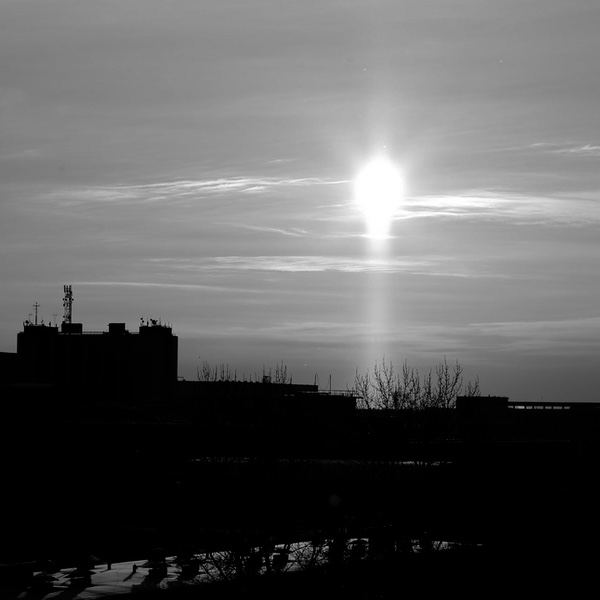
\includegraphics[width = 0.3\tw]{pillars}
	\caption{Солнечные столбы на восходе}
	\label{pic:pillars}    
\end{wrapfigure}
Это узкие столбы света, которые визуально исходят от Солнца вертикально вверх, а иногда и вниз. Их высота может достигать 5\,--\,$10^\circ$, а иногда и больше. Солнечные столбы не являются вертикальными лучами, на самом деле они представляют собой отражение Солнца в миллионах кристаллов льда. Иногда они выглядят как несколько вертикально расположенных световых пятен, в зависимости от расположения облачных кристаллов.

Солнечные столбы формируются пластинчатыми кристаллами, которые, дрейфуя в окологоризонтальном положении, отражают солнечный свет в вертикальной плоскости. Высота столбов определяется зависимостью коэффициента отражения от угла падения света на основания ледяных кристаллов и высотой Солнца над горизонтом, суть углом падения света на отражающую поверхность.



